\documentclass[11pt]{article}

\usepackage{setspace}
\usepackage{geometry}
\geometry{left=1in,right=1in,top=1in,bottom=1in}
\usepackage{graphics}
\usepackage{algorithmic}
\usepackage{algorithm}
\usepackage{epsfig}

\newtheorem{THM}{Theorem}[section]
\newtheorem{COR}{Corrolary}[section]
\newtheorem{PRF}{Proof}
\newtheorem{DEF}{Definition}[section]

\begin{document}

\bibliographystyle{plain}
\pagestyle{plain}
\pagenumbering{arabic}

\title{Unsupervised Study of Cell Behaviour for Breast Cancer}

\author{Supratim Bhattacharya,Jayanta Poray and Sampurna Mandal \\
Department of Computer Science \& Engineering, Techno India University,\\Saltlake, kolkata - 700091, India\\
E-mail:bhattacharya.supratim@gmail.com, jayanta.poray@gmail.com,piu.sampurna@gmail.com}

\maketitle

% --------------------------------------------------------------------------------------------------------------------
\begin{abstract}
Women's most threatened diseases is breast cancer.It is the leading cause of death for women today and it is the most common cancer in developed countries.Recently, the collection of biological data has been increasing at an ex-plosive rate. In this domain, Data Mining plays an important role.

\end{abstract}

% --------------------------------------------------------------------------------------------------------------------
\section{Introduction}
In India the event of breast cancer cases are increasing day by day. A new global study estimates that by 2030, the number of new cases of breast cancer in India will increase from the current 115,000 to around 200,000 per year.Cancer treatment and early successful diagnosis of the patients is a challenge since so many years. Doctors and Researchers have been working every day to find new ways to treat cancer.Data mining for cancer treatment can become a great support tool for doctors and physicians for decision making and estimation purpose. The need for biological data mining is that there is too much data but they are mostly unstructured.Data mining and machine learning depend on classification which is the most essential and important task. Many experiments are performed on medical datasets using multiple classifiers and feature selection techniques. A good amount of research on breast cancer datasets is found in literature. Many of them show good classification accuracy.

Data mining approaches in medical domains is increasing rapidly due to the improvement effectiveness of these approaches to classification and prediction systems, especially in helping medical practitioners in their decision making. In addition to its importance in finding ways to improve patient outcomes, reduce the cost of medicine, and help in enhancing clinical studies. Although there was a great deal of public education and scientific research, Breast cancer considered the most common invasive cancer in women, with more than one million cases and nearly 600,000 deaths occurring worldwide annually.Data mining and machine learning depend on classification which is the most essential and important task. Many experiments are performed on medical datasets using multiple classifiers and feature selection techniques. A good amount of research on breast cancer datasets is found in literature. Many of them show good classification accuracy.

We have applied WEKA machine learning technique to analyze the risk factors so that early diagnosis and proper preventive measures can be taken. We have used the Wisconsin Diagnostic Breast Cancer  Dataset from UC Irvine for our study. The classification is based on benign or malignant.
%------------------------------------------------




%
\section{Problem Definition}
The dataset used in this experiment were obtained from Wisconsin Diagnostic Breast Cancer Dataset from UC Irvine machine learning repository and described by Dr. William H. Wolberg. The breast cancer data have been used in some other research. We study the effect of nine characteristics parameter on the state of Breast cancer and the influence of the involved parameters on the performance of the SVM model. We have used WEKA Tool as a classifier in our experiment. Our aim is to predict the various state, behaviour and characteristics of breast cancer.

In this dataset, there are 698 samples taken from different women and every sample is expressed by nine characteristic parameter. The nine parameter are as follows:- Clump thickness, Uniformity of cell size, Uniformity of cell shape, Marginal adhesion, single epithelia cell size, Bare Nuclei, Bland chromatic, Normal Nucleoli, Mitoses. According to the properties of these nine parameter, the brest cancer is classified into benign \& malignant. Every single parameter is given a range between 1 to 10 and the resultant class is expressed by 2 for benign and 4 for malignant. Among the 698 samples in the dataset there are 16 samples with missing or incomplete data. So we have used remaining 682 samples in this machine learning.

\section{Proposed Model}

Fig 1 shows the functional block diagram of our proposed model. It consists of four steps: (a) Acquisition, (b) Preprocess, (c) Feature Extraction and (d) Feature Selection.

In acquisition step, feature selection \& feature extraction is accomplished in order to determine the input vector and based on either feature selection or feature extraction, dimensionality reduction is accomplished. In the preprocessing phase, filtering is done to clear the noise \& map the entire data into lower dimension. Also less important and redundant information are ignored. In the classification step different classifier is used to get the best result out of it. We have also applied clustering method \& Association Rule Mining to obtain more decisions \& to predict more accurately
\section{Methodology}

The dataset's attributes are found listed in Table 2.
\vspace{.5 cm}
 \begin{center}
     \textbf{Table2: WISCONSIN BREAST CANCER DATASET ATTRIBUTES}
   \end{center}

    \begin{tabular}{|c|c|c|}
      \hline
      & Attribute & Domain\\
      \hline
      1 & Sample Code No & id no\\
      \hline
      2 & Clumb Thickness & 1-10\\
      \hline
      3 & Uniformity(Cell Size) & 1-10\\
      \hline
      4 & Uniformity(Cell Shape) & 1-10\\
       \hline
      5 & Marginal Adhesion & 1-10\\
       \hline
      6 & sgl Epithelial(cell size) & 1-10\\
       \hline
      7 & Bare Nucleoli & 1-10\\
       \hline
      8 & Normal Nucleoli & 1-10\\
       \hline
      9 & Mitoses & 1-10\\
       \hline
      10 & Class & 2 or 4\\
      \hline
    \end{tabular}

\vspace{.5 cm}
In the Clump thickness benign cells tend to be grouped in monolayers, while cancerous cells are often grouped in
multilayered. While in the Uniformity of cell size/shape the cancer cells tend to vary in size and shape. That is why these parameters are valuable in determining whether the cells are cancerous or not. In the case of Marginal adhesion the normal cells tend to stick together, where cancer cells tend to lose this ability. So loss of adhesion is a sign of malignancy. In the Single epithelial cell size the size is related to the uniformity
mentioned above. Epithelial cells that are significantly enlarged may be a malignant cell. The Bare nuclei is a term used for nuclei that is not surrounded by cytoplasm (the rest of the cell). Those are typically seen in benign tumors. The Bland Chromatin describes a uniform "texture" of the nucleus seen in benign cells. In cancer cells the chromatin tends to be coarser. The Normal nucleoli are small structures seen in the nucleus. In normal cells the nucleolus is usually very small if visible. In cancer cells the nucleoli become more prominent, and
sometimes there are more of them. Finally, Mitoses is nuclear division plus cytokines and produce two identical daughter cells during prophase. It is the process in which the cell divides and replicates. Pathologists can determine the grade of cancer by counting the number of mitoses.


We next present our algorithm and further describe the dataset on which we have evaluated.

our first step is to discretize the dataset into three major groups.
\begin{enumerate}
\item Low
\item Mid
\item High
\end{enumerate}

\begin{algorithm}[H]
\caption{An algorithm for discretization  of dataset}


\textbf{Input} : Dataset in excel format with $9$ parameters.

\textbf{Output:} : Dataset in csv file(space delimiter) format in discrete format with all $9$ parameters.

\textbf{Algorithmic Steps:}
\begin{enumerate}
  \item Obtain the ranges of high, middle and low.
  \item collect every cell value for computation for every parameter.
  \item \textbf{For} parameter $1$ to $9$ do
  \item \textbf{If} Cell value>= high value \textbf{Then}
            \textbf{Put} new Cell value= 'H'
            \textbf{Else If} Cell value>= middle value \textbf{Then}
             \textbf{Put} new Cell value= 'M'
             \textbf{Else}
             \textbf{Put} new Cell value= 'L'
  \item \textbf{End if}
  \item \textbf{Next}
  \item \textbf{For} $10^th$ parameter
  \item \textbf{If}Cell value=2 \textbf{Then}
  \item \textbf{Put} new Cell value = "Benign"
  \item \textbf{Else If}Cell value=4 then
  \item \textbf{Put}new Cell value = "Malignant"
  \item \textbf{End If}
  \item Construct another excel file based on this discrete value.
  \item Convert the excel file into csv(space delimiter) file.
\end{enumerate}

\end{algorithm}



As the parameter of the dataset ranges from 1 to 10 we made this discretization based on different ranges like:-

\begin{enumerate}
\item low:- 1 to 1 mid:- 2 to 6 high:- 7 to 10
\item low:- 1 to 1 mid:- 2 to 7 high:- 8 to 10
\item low:- 1 to 2 mid:- 3 to 7 high:- 8 to 10
\item low:- 1 to 3 mid:- 4 to 6 high:- 7 to 10
\item low:- 1 to 4 mid:- 5 to 6 high:- 7 to 10
\item low:- 1 to 4 mid:- 5 to 7 high:- 8 to 10
\end{enumerate}

 --------------------------------------------------------------------------------------------------------------------
\section{Methods}




% --------------------------------------------------------------------------------------------------------------------
\section{Analytical framework}
Cancer cell description:The breast cell attributes behavior can be helpful in determining whether the cell is normal or cancerous.Some cells can be visualized like in given figure-2.In the figure it is seen that the nucleoli in normal cell is approximately invisible but the cancerous cell has an enlarged one.In the mitosis attribute the cell division is so fast and uncontrolled then the cell size and shape varies a lot in the cancerous cell.Then according to the bare nuclei attribute, a cancerous cell is comparatively dry.  
\begin{figure}[!h]
\centering
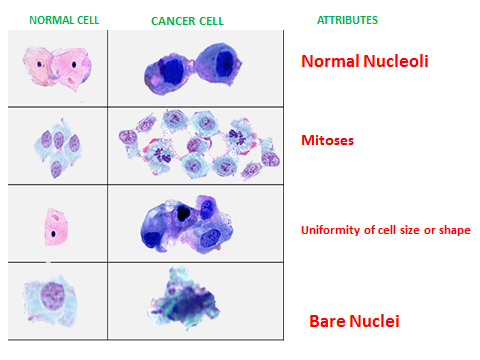
\includegraphics[scale=0.7]{attri}
\caption{normal vs cancerous cell attributes'behavior}
\label{fig_sin}

\end{figure}
Decision tree-Decision tree is a popular classification method.Decision tree is used as a predictive model which maps observations about an item to conclusions about the item's target value.Rules produced by decision tree induction are easy to interpret and understand and hence can help greatly in appreciating the underlying mechanism that separate samples in different classes.One of the decision tree algorithms is c4.5.C4.5 builds decision trees from a set of training data using the concept of information entropy.It uses the information gain ratio criterion to determine the most discriminatory feature at each step of its  decision tree induction process.Pruning helps to reduce the size of decision trees by removing sections of the tree that provide little power to classify instances.Pruning reduces the complexity of the final classifier and hence improves predictive accuracy by the reduction of over fitting.
\begin{figure}[!h]
\centering
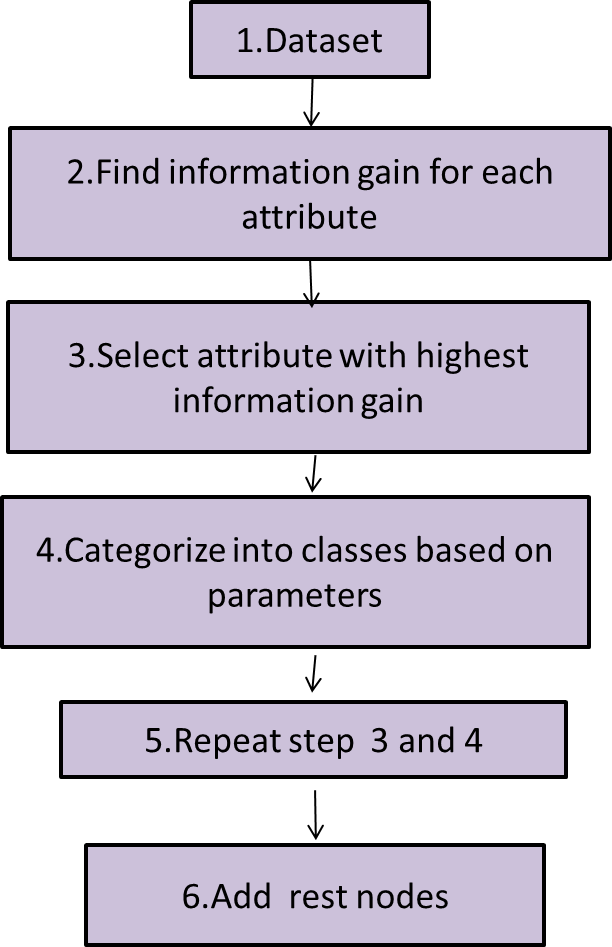
\includegraphics[scale=0.7]{c45}
\caption{flowchart of c4.5}
\label{fig_sin}
\end{figure}
Algorithm:
Step 1.The leaf is labelled with the same class if the instances belong to the same class. 
Step 2: For every attribute, the potential information will be calculated and the gain in information will be taken from the test on the attribute. 
Step 3: Finally the best attribute will be selected based on the current selection parameter.

FORMULa
Association Rules Mining
Since its introduction in 1993[1] the task of association rules mining has received a great deal of attention.Association Rules mining is the datamining process of finding the rules that may govern associations and causal objects between sets of items.It is used to find out association rules that satisfy the predefined minimum support and confidence from a given database.The problem is usually decomposed into two subproblems.One is to find those item sets whose occurrences exceed a predefined threshold in the database;those item sets are frequent or large item sets.The second problem is to generate association rules from those large item sets with the constriants of minimal confidence.
One of the popular algorithms is the aprioiri algorithm.Its iteravely reduces the minimum support until it finds the required number of rules with the given minimum confidence.
The algorithm has an option to mine class association rules.
Mathematical formulae-   
 


% --------------------------------------------------------------------------------------------------------------------
\section{Discussion}

 
% --------------------------------------------------------------------------------------------------------------------
\section{Results}


Based on these cell's behavior the dataset's attributes values can largely help in determination and diagnosis.On discretisation and preprocessing,each attribute shows its own graphical result divided into 3 bins based on high,medium and low values. Fig-3 shows normal nucleoli attribute and the no. of patient instances classified into benign and malignant group. The figure shows that out of 509 instances with low or small value has 30% 

 
\begin{figure}[!h]
\centering
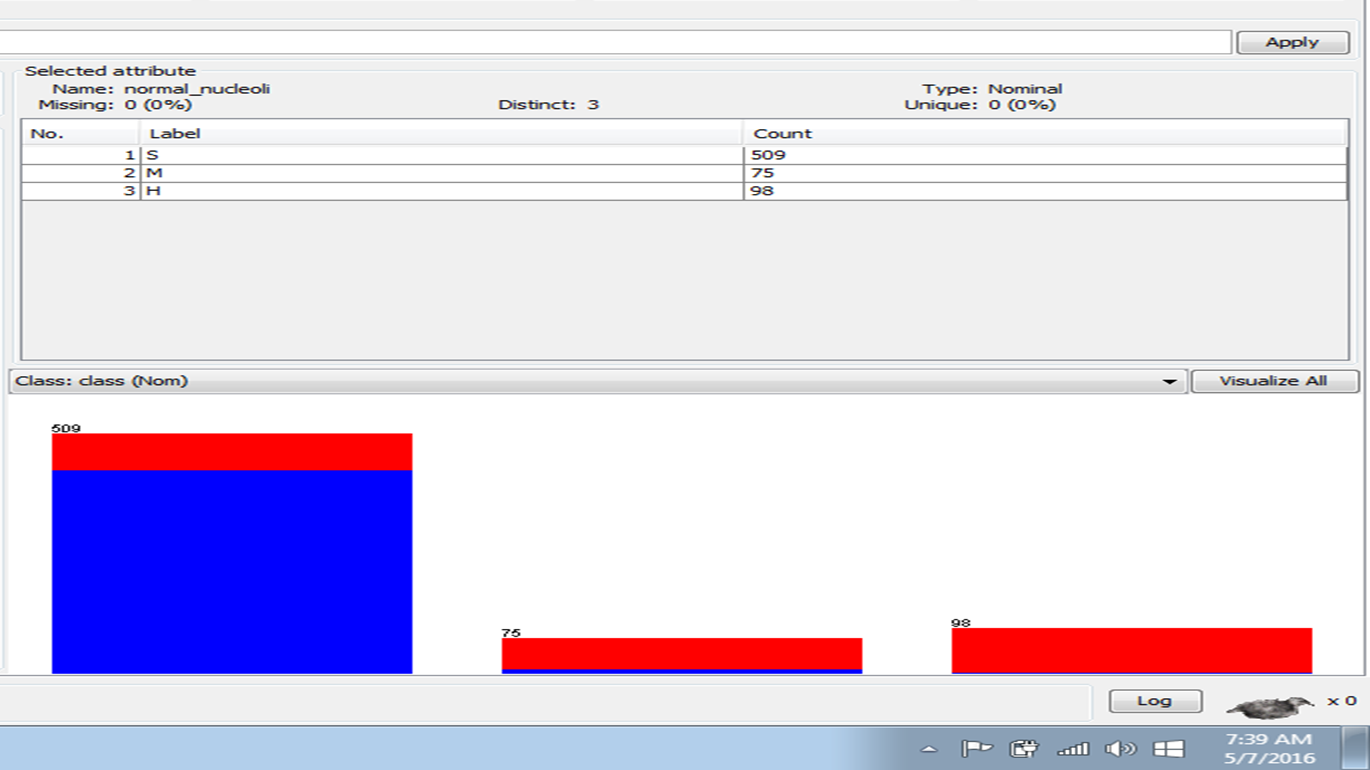
\includegraphics[scale=0.4]{nucleifig}
\caption{normal nucleoli}
\label{fig_sin}

\end{figure}
Similarly all attributes can be visualised at a time shown in figure below. 
\begin{figure}[!h]
\centering
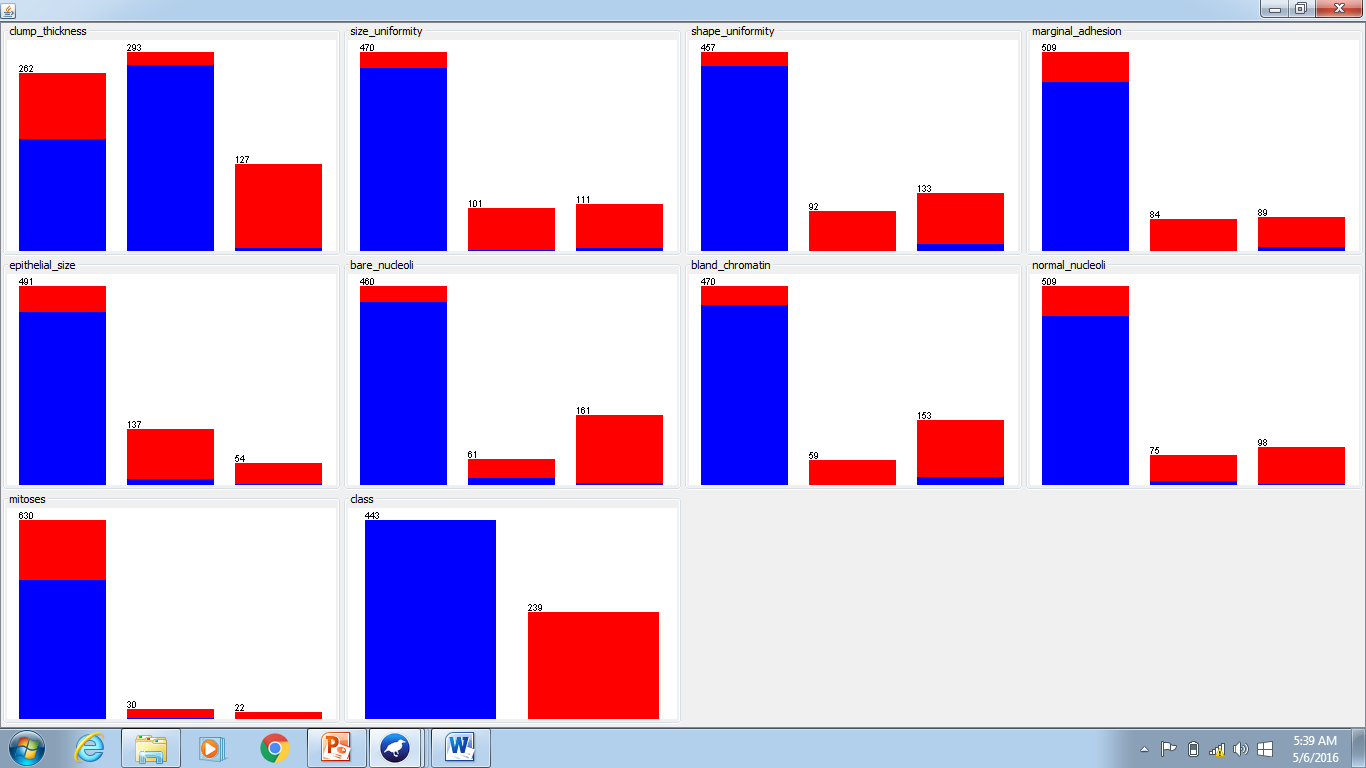
\includegraphics[scale=0.3]{visuals}
\caption{All attributes}
\label{fig_sin}

\end{figure}



\begin{figure}[!h]
\centering
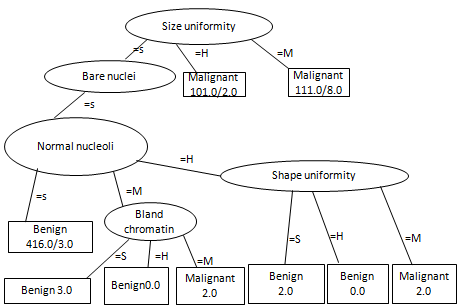
\includegraphics[scale=0.7]{tree}
\caption{Decision tree}
\label{fig_sin}

\end{figure}

malignant and 70% 
benign then out of 75 instances with medium value 90% 
are Malignant and 10% 
Benign then out of 98 instances with high value 99% 
are Malignant and 1% 
benign.According to the observation  the higher the value of the attributes the greater the tendency towards malignancy.
On observing the J48 pruned tree and considering only the malignant category  we can see that a combination of two medium values or one high and another medium value or only high values can help in determining malignancy.
Selection of the most useful attribute is necessary.Information gain evaluator can help to find the attribute highest priority.The output presented below shows information gain values of each and every attribute and their ranking.FIGURE Size uniformity is selected as the best one.Then shape uniformity and so on.On selecting a set of attributes based on the ranking we get one or different kinds of rules.Among them the best and of utmost importance are selected.
the table below shows different statistical measures.Kappa statistics,
mean absolute errorand others have their own significance and importance.Studies that measure the argument between two or more observers that takes into account the fact that observers will sometimes agree or disagree simply by chance.The calculation is based on the difference between how much agreement is acyually present (observed agreement)compared to how much agreement would be expected to be  present by chance alone (expected agreement).The MAE and RMSE can be used together to diagnose the variation in the errors in a set of forecasts.The RMSE will always be larger or equal to the MAE;The greater the difference between them  the greater the variance in the individual errors in the sample.If RMSE=MAE then all the errors are of the same magnitude.


\begin{figure}[!h]
\centering
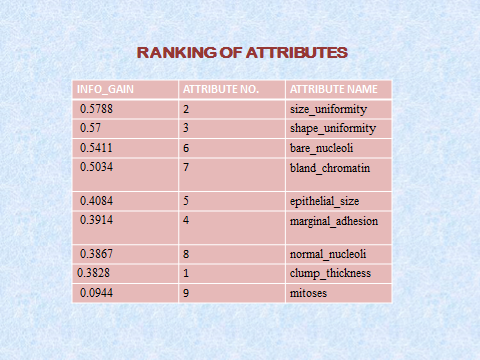
\includegraphics[scale=0.7]{rankingg}
\caption{ranking}
\label{fig_sin}

\end{figure}
\begin{figure}[!h]
\centering
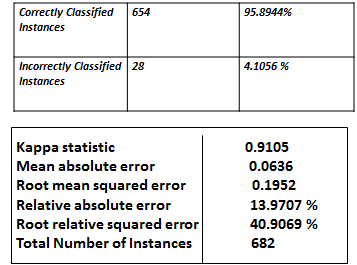
\includegraphics[scale=0.7]{classification}
\caption{classification results}
\label{fig_sin}

\end{figure}



% --------------------------------------------------------------------------------------------------------------------
\bibliography{Reference}
% --------------------------------------------------------------------------------------------------------------------
\newpage
% --------------------------------------------------------------------------------------------------------------------
\textbf{APPENDIX}





Pearson correlation coefficient between two expression vectors $X$ and $Y$ is computed
as,
\begin{equation}\label{Correlation}
\rho =\frac{cov(X,Y)}{\sigma_{X}\sigma_{Y}}
=\frac{\sum_{i=1}^N(x_{i}-\overline{x})(y_{i}-\overline{y})}
{\sqrt{[\sum_{i=1}^N(x_{i}-\overline{x})^{2}][\sum_{i=1}^N(y_{i}-\overline{y})^{2}]}}.
\end{equation}

Suppose, an event is observed n times out of total N observations and given the evidence that the event originally occurs e times out of E total cases. Then, the p-value is computed assuming a hypergeometric distribution as given follows.
\begin{equation}
p-value = \sum_{i=n}^{N} \frac{{e \choose i} {E-e \choose N-i}}{{E \choose N}}.\nonumber
\end{equation}

Supplementary Link: http://www.isical.ac.in/$\sim$malay\_r/Supplementary.html.

\end{document}
